\chapter{Conformer searches with CREST: from one structure to a refined ensemble}
\chaptermark{Conformer searches with CREST}
\label{ch:crest}
\index{CREST}
\index{Conformer search}
\index{Boltzmann weights}
\index{Coupled codes}
\checkedwith{9.5.3-dev}{d26701ae0}
\helppage{crest}

A molecule that can rotate about its single bonds has no single structure, and the structure we draw is one point on a surface with many minima. Whether it matters which minimum we compute depends on the question. For a rigid aromatic ring it does not, whereas for a flexible chain with a donor and an acceptor for a hydrogen bond it decides the energy, the dipole moment, the NMR couplings and, further down the road, the binding to a protein. In this chapter we search for the minima with CREST, read the resulting ensemble in ECCE, and decide which of its members deserve a more expensive calculation. The example is 2-methoxyethanol, \chem{CH3OCH2CH2OH}, a molecule small enough for the search to take three minutes and flexible enough to show what an ensemble looks like.

\section{Background}
\index{Conformers!when they matter}\index{Intramolecular hydrogen bonds}\index{Ring puckers}\index{Rotamers}

A conformer is a minimum of the energy surface that differs from the others by rotation about single bonds or, in a ring, by a change of pucker. Conformers matter whenever the energy differences between them are comparable to $RT$, which is $0.59$~kcal/mol at 298~K, since the measured property is then an average over several structures. The cases an organic chemist meets most often are the chair and twist-boat forms of rings and the axial or equatorial position of a substituent, the rotamers of an alkyl chain, the \emph{cis} and \emph{trans} forms of an amide or ester, and any molecule in which a donor and an acceptor can reach each other, so that the internal hydrogen bond competes with the extended chain.

2-Methoxyethanol has two rotations that set this competition. About the central C--C bond the two oxygen atoms are either \emph{gauche}, which lets the hydroxyl hydrogen reach the ether oxygen in a five-membered ring, or \emph{anti}, which keeps them apart. The C--O bonds add further rotamers of the hydroxyl and the methyl group. A person looking at a drawing would guess the \emph{gauche} form with the hydrogen bond, and the search tells us how much of the ensemble that guess accounts for.

CREST \cite{pracht2020} finds the minima by running short metadynamics trajectories from the input structure, which push the molecule over rotational barriers, optimising the snapshots and sorting out duplicates. Since the trajectories and the optimisations use a tight-binding method, GFN2-xTB \cite{bannwarth2019} or the force field GFN-FF \cite{spicher2020}, the search takes minutes for a molecule of this size and hours for a drug-sized one, where a density functional calculation on every starting structure would not be possible. The price is that the energies of such methods order conformers only roughly, and the chapter returns to that when we choose what goes on to a better level.
\index{GFN2-xTB}\index{GFN-FF}\index{Metadynamics}

\section{What ECCE shows}
\index{CREST!run types}\index{Run types!CREST}

The \menu{CREST} button in the code bar makes a calculation with this code. CREST runs \cmd{xtb} itself, so both programs are registered for the machine in \menu{Register Machines}, and the xTB path of the machine is the one CREST uses. Four run types are offered. \menu{Conformer Search} is the one of this chapter. \menu{Protonation Sites} adds a proton at every basic site of the molecule and returns the protonated structures, lowest first, and \menu{Tautomers} moves protons between the sites; both work with GFN2-xTB only and have an energy window of 30~kcal/mol, and Chapter~\ref{ch:protonation} puts them to use. \menu{Solvation Shell} grows a cluster of solvent molecules around the solute, the subject of Chapter~\ref{ch:pom-solvation}.
\index{CREST!Protonation Sites}\index{CREST!Tautomers}\index{CREST!Solvation Shell}

The \menu{Theory} of a conformer search is \menu{GFN2-xTB}, the default; \menu{GFN-FF}, which is much faster and suits a first look at a large floppy system; or \menu{GFN2//GFN-FF}, which searches with the force field and re-optimises and ranks with GFN2-xTB. The \menu{Theory Details} offer an implicit solvent, ALPB or GBSA, and \menu{Runtype Details} the \menu{Energy window} in kcal/mol (6 by default), which sets how far above the lowest conformer a structure may lie and still be kept. Two options exist for special cases. \menu{Non-covalent complex (NCI mode)} keeps the parts of a host--guest complex together, and the two topology options (\menu{Skip the reference-topology check} and \menu{No topology check}) stop CREST from discarding structures whose bonds it reads differently from the input, which happens for ion clusters.
\index{CREST!Energy window}\index{CREST!Theory}\index{Implicit solvent!ALPB}\index{ALPB}\index{CREST!NCI mode}

CREST has to start from an optimised structure. An xTB geometry optimisation is therefore the first calculation, and the Launch of a CREST calculation warns when it does not follow one (\menu{Launch anyway} goes on).
\index{CREST!starting structure}

\section{Procedure}
\index{Tools menu!Add from SMILES...}\index{SMILES}

Everything happens in one project folder of the Organizer, so that each calculation can take its structure from the one before.
\begin{enumerate}
	\item With \menu{File > New} make an xTB calculation. In the Builder choose \menu{Tools > Add from SMILES...}, enter \texttt{COCCO}, and set the run type to Geometry with the theory GFN2-xTB. Launch it.
	\item Click the \menu{CREST} button in the code bar to make a CREST calculation, and give it the structure of the xTB result. Choose the run type \menu{Conformer Search} and the theory \menu{GFN2-xTB}, leave the \menu{Energy window} at 6~kcal/mol, and launch it with four cores in the Launcher.
	\item For the second search make a copy of the CREST calculation and set the implicit solvent in \menu{Theory Details} to ALPB, solvent water. Launch it.
	\index{CREST!Implicit Solvent}
	\item When a search is complete, open it in the Builder and choose \menu{Properties > Geometry > Conformers}. The columns can be sorted, \menu{Export .csv...} saves the table and \menu{Export .png...} the table with its pictures.
	\item To compare structures, Ctrl-click several rows. The Builder fits them onto the first one clicked, and the key below the table lists the colour of each member and its heavy-atom RMSD to that reference.
	\index{Conformers panel!Superposing members}\index{RMSD}
	\item To refine the conformers worth keeping, select their rows and choose \menu{New Calculation from Selected...}, which asks once for the code and makes one geometry optimisation for each, named after the CREST calculation with \texttt{\_conf} and the rank.
	\index{Conformers panel!New Calculation from Selected}
\end{enumerate}

We made the calculations of this chapter headless, through ECCE's own Launch with the decks that the same scripts write for the Calculation Editor, in an isolated data folder (ECCE 9.5.3-dev, \cmd{nice} level 19, four cores). The harness stores the structure and deck of each calculation and not the Calculation Editor setup, and the starting structure came from Open Babel with the same SMILES string. The Organizer and Builder steps follow the help pages and were driven through the windows only as far as opening the \menu{Conformers} panel.

\section{Results}
\index{2-Methoxyethanol}

\subsection{The ensemble}
The xTB optimisation took 40~s, the GFN2-xTB search 193~s on four cores. CREST kept 16 conformers within 6~kcal/mol, of which the first eight are in Table~\ref{tab:crest-gas} together with two measures that we read from the stored coordinates, the O--C--C--O dihedral and the distance from the hydroxyl hydrogen to the ether oxygen. Figure~\ref{fig:crest-table} shows the same list in the \menu{Conformers} panel.
\index{Boltzmann weights!Conformers panel}

\begin{table}[htb]
	\centering
	\caption{The eight lowest conformers of 2-methoxyethanol from the GFN2-xTB search in the gas phase. $\Delta E$ is relative to the lowest conformer of this search, the weight is the Boltzmann population at 298.15~K, $\tau$ the O--C--C--O dihedral and $d$ the H$\cdots$O distance from the hydroxyl hydrogen to the ether oxygen.}
	\label{tab:crest-gas}
	\begin{tabular}{rrrrr}
		\toprule
		Rank & $\Delta E$ (kcal/mol) & Weight (\%) & $\tau$ (\si{\degree}) & $d$ (\si{\angstrom}) \\
		\midrule
		1 & 0.000 & 48.9 & 63 & 2.40 \\
		2 & 0.373 & 26.0 & $-58$ & 2.35 \\
		3 & 1.118 & 7.4 & 172 & 3.87 \\
		4 & 1.499 & 3.9 & $-82$ & 3.53 \\
		5 & 1.586 & 3.4 & 178 & 3.89 \\
		6 & 1.665 & 2.9 & 169 & 3.95 \\
		7 & 1.777 & 2.4 & 45 & 2.60 \\
		8 & 2.205 & 1.2 & $-96$ & 3.11 \\
		\bottomrule
	\end{tabular}
\end{table}

\begin{figure}[htb]
	\centering
	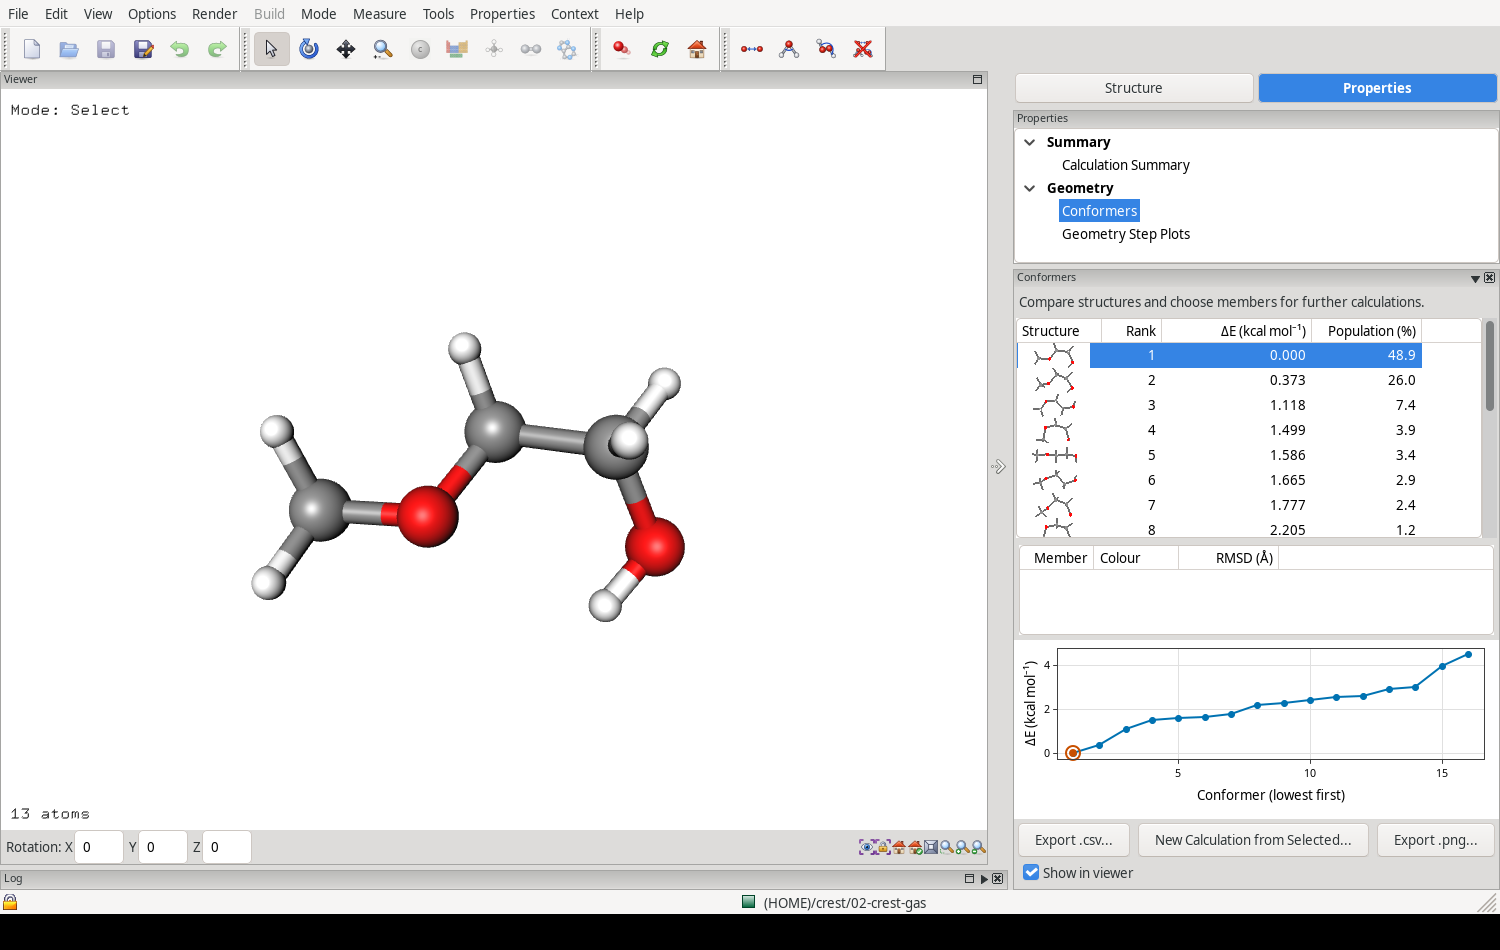
\includegraphics[width=\linewidth]{crest/conformers-gas.ecce-9.5.3-dev.png}
	\caption{The \menu{Conformers} panel for the gas-phase search on 2-methoxyethanol. The table lists rank, relative energy and population, the plot below it the energy against the rank, and the 3-D view shows the lowest conformer on a white background.}
	\label{fig:crest-table}
\end{figure}

The two lowest conformers are \emph{gauche} about the central bond, with the hydroxyl hydrogen \SI{2.40}{\angstrom} and \SI{2.35}{\angstrom} from the ether oxygen, and in the lowest the O$\cdots$O distance is \SI{2.84}{\angstrom}. They are five-membered rings closed by the hydrogen bond. Taken together with rank 7, the only other conformer with a hydrogen to oxygen distance below \SI{2.6}{\angstrom}, they carry 77~percent of the weight of the ensemble. Ranks 3, 5, 6, 11 and 12 are \emph{anti}, with the two oxygens on opposite sides, and carry 15~percent. Rank 4 is \emph{gauche} as well, but with the hydroxyl turned away, which shows that the \emph{gauche} arrangement alone does not make the bond.

The first two conformers differ by 0.37~kcal/mol, which is below what a tight-binding method resolves, so we treat them as one group and not as a ranking. Superposing ranks 1, 2 and 3 (Fig.~\ref{fig:crest-overlay}) shows what the numbers describe: the heavy-atom RMSD of rank 2 to rank 1 is \SI{0.55}{\angstrom}, since both have the same ring of five atoms and differ in the orientation of the methyl group and the hydroxyl, whereas rank 3, with the chain extended, lies \SI{0.84}{\angstrom} away.

\begin{figure}[htb]
	\centering
	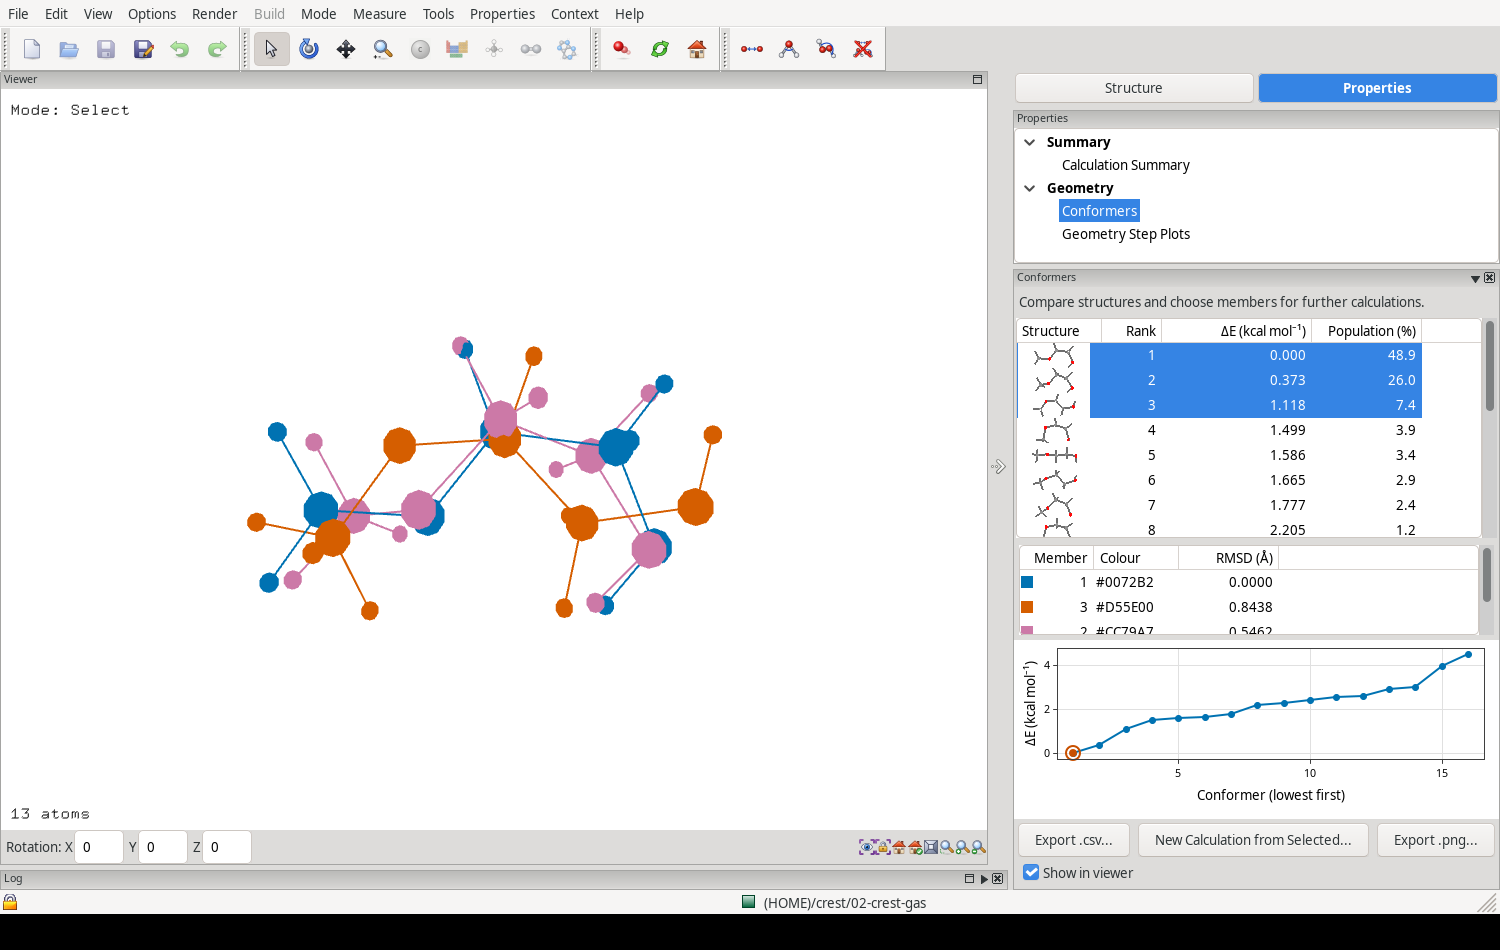
\includegraphics[width=\linewidth]{crest/conformers-overlay.ecce-9.5.3-dev.png}
	\caption{Ranks 1, 2 and 3 of the gas-phase search, fitted onto rank 1 (blue). The key under the table gives the heavy-atom RMSD of each member to the reference.}
	\label{fig:crest-overlay}
\end{figure}

\subsection{The same search with implicit water}
The second search, with ALPB water, took 201~s and also kept 16 conformers. Its lowest structure is again a \emph{gauche} conformer with the hydrogen bond (the hydrogen to oxygen distance is \SI{2.53}{\angstrom}), but the weight of the conformers with a hydrogen to oxygen distance below \SI{2.6}{\angstrom} falls from 77 to 50~percent, and that of the \emph{anti} conformers rises from 15 to 29~percent. We read this as a comparison of structures within each search. The energies of the two searches belong to different models and are not subtracted from one another. The implicit solvent also treats water as a continuum, so the shift tells us that a polar medium weakens the preference for the internal bond, and it cannot tell us what the explicit hydrogen bonds to water molecules do. For that the \menu{Solvation Shell} run type of Chapter~\ref{ch:pom-solvation} is the tool.

One sentence is what the example shows chemically: in the gas phase about three quarters of 2-methoxyethanol sits in a hydrogen-bonded ring, and a continuum model of water already moves a good part of that weight to the extended forms.

\subsection{What to take on}
Before going further we have to decide how many conformers justify a better calculation. The ranking of a tight-binding method is not reliable to a few tenths of a kcal/mol, which means that a cut at the lowest conformer would be a gamble. Chapter~\ref{ch:coupling} shows this for ibuprofen, where the conformer that the best method puts first is the fourth of the cheap one, and it recommends passing on every conformer within the uncertainty of the cheap method and a few more besides. Here the weights give a natural choice. The eight conformers of Table~\ref{tab:crest-gas} carry 96~percent of the ensemble, and since several of them differ only by a methyl rotation, \cmd{ecce-ensemble pick} would merge them into the distinct structures before we spend any density functional time. We ran no higher level for this chapter. For the ranking of the structures at that level, Chapter~\ref{ch:coupling} gives the route and the table to compare.
\index{Funnel!choice of the number of structures}\index{Commands!ecce-ensemble}\index{Distinct conformers}

Re-optimising the lowest conformer with GFN2-xTB at the tight level (35~s) left the structure unchanged, which we expected, since CREST uses the same method; an xTB step after a GFN2 search therefore adds nothing, whereas after a GFN-FF search it moves the structures to the minima of the better method.

The calculations are in the repository of this book under \texttt{calculations/crest}.

\section{Coupling with other codes}
\index{Coupling!CREST}

CREST sits at the head of the funnel of Chapter~\ref{ch:coupling}. What feeds it is an optimised structure, and that comes from xTB or from any other code, since a finished calculation hands over its final geometry together with its charge and multiplicity. For a larger molecule the search can start with GFN-FF for a first look, and \menu{GFN2//GFN-FF} does the force-field search and the GFN2-xTB ranking in one calculation at a higher cost.

What the search feeds is the ensemble. \menu{New Calculation from Selected...} starts one calculation per conformer in another code, typically an xTB optimisation and then a density functional calculation in ORCA, and \cmd{ecce-series} does the same for a longer list from a template. We make these hand-offs by hand, since a few conformers do not justify automation. A workflow pays when the chain recurs, as for the protonation sites of an aminopyridine, where CREST, xTB and ORCA run as one unit (Chapter~\ref{ch:workflows}). The structures of the ensemble can also go the other way, towards the solvent: the lowest conformers are the starting points of the solvation shell calculations of Chapter~\ref{ch:pom-solvation}, and \menu{Protonation Sites} and \menu{Tautomers} (Chapter~\ref{ch:protonation}) use the same panel and the same hand-offs for ions and isomers.
\index{New Calculation from Selected}\index{Commands!ecce-series}\index{Workflows}
